\documentclass[12pt, a4paper]{report}


\usepackage[utf8]{inputenc}
\usepackage[T1]{fontenc}
\usepackage[french]{babel}
\usepackage{graphicx}
\usepackage{geometry}
\usepackage{hyperref}
\usepackage[acronym]{glossaries}
\usepackage{subcaption}
\usepackage{xcolor}
\usepackage{colortbl}
\usepackage{gensymb}
\usepackage{wrapfig}
\usepackage{multicol}
\usepackage{fancyhdr}
\usepackage{booktabs}
\usepackage{eurosym}
\usepackage{titlesec}
\usepackage{subcaption}
\usepackage{tabularx}        % Tableaux à largeur ajustable
\usepackage[backend=biber, style=authoryear]{biblatex}
\pagestyle{fancy}
\fancyhf{}
\fancyfoot[C]{\thepage}

\addbibresource{references.bib}
\setlength{\bibitemsep}{5mm}

\renewcommand{\thechapter}{\Roman{chapter}} % Numérotation romaine

\usepackage{titlesec}
\titleformat{\section}
    {\normalfont\Large\bfseries\raggedright} % Ajoute \raggedright ici
    {\thesection}{1em}{}
\titleformat{\subsection}
    {\normalfont\large\bfseries\raggedright} % Ajoute \raggedright ici
    {\thesubsection}{1em}{}

% Redéfinir le style du chapitre : numéro + tiret + titre sur la même ligne
\titleformat{\chapter}
    {\normalfont\LARGE\bfseries} % Style du texte
    {\thechapter~--~} % Numéro romain suivi d'un tiret et d'un espace
    {0pt} % Espace entre le numéro et le titre (0pt car le tiret est déjà inclus)
    {} % Pas de texte supplémentaire

% Réduire l'espace avant et après le titre
\titlespacing*{\chapter}
    {0pt} % Espace horizontal à gauche
    {0pt} % Espace vertical avant le titre
    {1em} % Espace vertical après le titre

\setlength{\parindent}{0pt}


\definecolor{lightgray}{RGB}{220,220,220}
\definecolor{linkblue}{HTML}{00008B} % Bleu foncé standard
\colorlet{linkcolor}{linkblue!50} % Bleu foncé avec 50% d'opacité
\definecolor{excelHeader}{RGB}{31, 78, 121}     % Bleu foncé (En-tête)
\definecolor{excelBlue}{RGB}{217, 225, 242}     % Bleu clair (Constantes / Entrées fixes)
\definecolor{excelGreen}{RGB}{226, 239, 218}    % Vert clair (Variables de conception)
\definecolor{excelYellow}{RGB}{255, 242, 204}   % Jaune clair (Valeurs calculées / Sorties)
\definecolor{excelOrange}{RGB}{252, 228, 214}   % Orange clair (Contraintes / Limites)

% Redéfinir la commande \glslink pour les acronymes
\renewcommand*{\glslink}[2]{%
    \ifglsused{#1}{%
        \href{\glsrefanchor{#1}}{\colorbox{white}{\color{black}#2}}% Style pour les acronymes déjà utilisés
    }{%
        \href{\glsrefanchor{#1}}{\fboxsep=0pt\colorbox{acronymlinkcolor!20}{\color{black}#2}}% Style pour la première utilisation
    }%
}


\makeglossaries

%%%%% Defining Glossary Entries
\newglossaryentry{keyword}{
name={Name},
description={description}}



%%%%% Definition of Acronyms
\newacronym{ipsa}{IPSA}{Institut Polytechnique des Sciences Avancées}
\newacronym{ml}{ML}{Machine Learning}
\newacronym{swx}{SWx}{Space Weather}
\newacronym{onera}{ONERA}{Office National d'Études et de Recherches Aérospatiales}




% Marges et mise en page
\geometry{
    a4paper,
    left=25mm,
    right=25mm,
    top=25mm,
    bottom=25mm,
}


\hypersetup{
  colorlinks      = false,
  urlbordercolor  = red,     % cadre rouge pour \url et \href
  linkbordercolor = white,   % cadre "invisible" pour \gls, \acrshort,   
  citebordercolor = blue,    % cadre "bleu" pour la biblio
  filebordercolor = white,
}


\begin{document}

% Largeur commune des logos : en fixant une valeur absolue (cm),
% les deux logos auront exactement la même largeur à l'affichage,
% quelle que soit la résolution ou le ratio de l'image source.
\newcommand{\logowidth}{3.2cm}

\begin{titlepage}
    \centering
    \vspace*{-1.2cm} % remonte l'ensemble du bloc de logos vers le haut de la page

    % ---- Ligne des logos (alignés en haut grâce à [t]) ----
    \noindent
    \begin{minipage}[t]{0.48\textwidth}
        \raggedright
        
\includegraphics[width=\logowidth]{logos/IPSA_LOGO_2024_QUADRI.png}\\[0.3cm]
        \textbf{\textsc{Institut Polytechnique des Sciences Avancées}} \\
        \small 81 Av. de Grande-Bretagne \\
        \small 31300 Toulouse, France 
    \end{minipage}
    \hfill
    \begin{minipage}[t]{0.48\textwidth}
        \raggedleft
        
\includegraphics[width=6.5cm]{logos/ONERA_logo.png}\\[0.3cm]
        \textbf{\textsc{Office National d'Études et de Recherches Aérospatiales}}\\
        \small 2 Av. Marc Pélegrin,  \\
        \small 31400 Toulouse, France
    \end{minipage}

    \vspace{1.2cm}

    % ---- Titre du rapport ----
    {\Large \textbf{Rapport PMI}} \\
    \vspace{0.5cm}
    {\Huge \textbf{Reconstitution de données d'environnement spatial}}
    \vspace{5mm}

    % ---- Image centrale ----
    \begin{figure}[h]
        \centering
        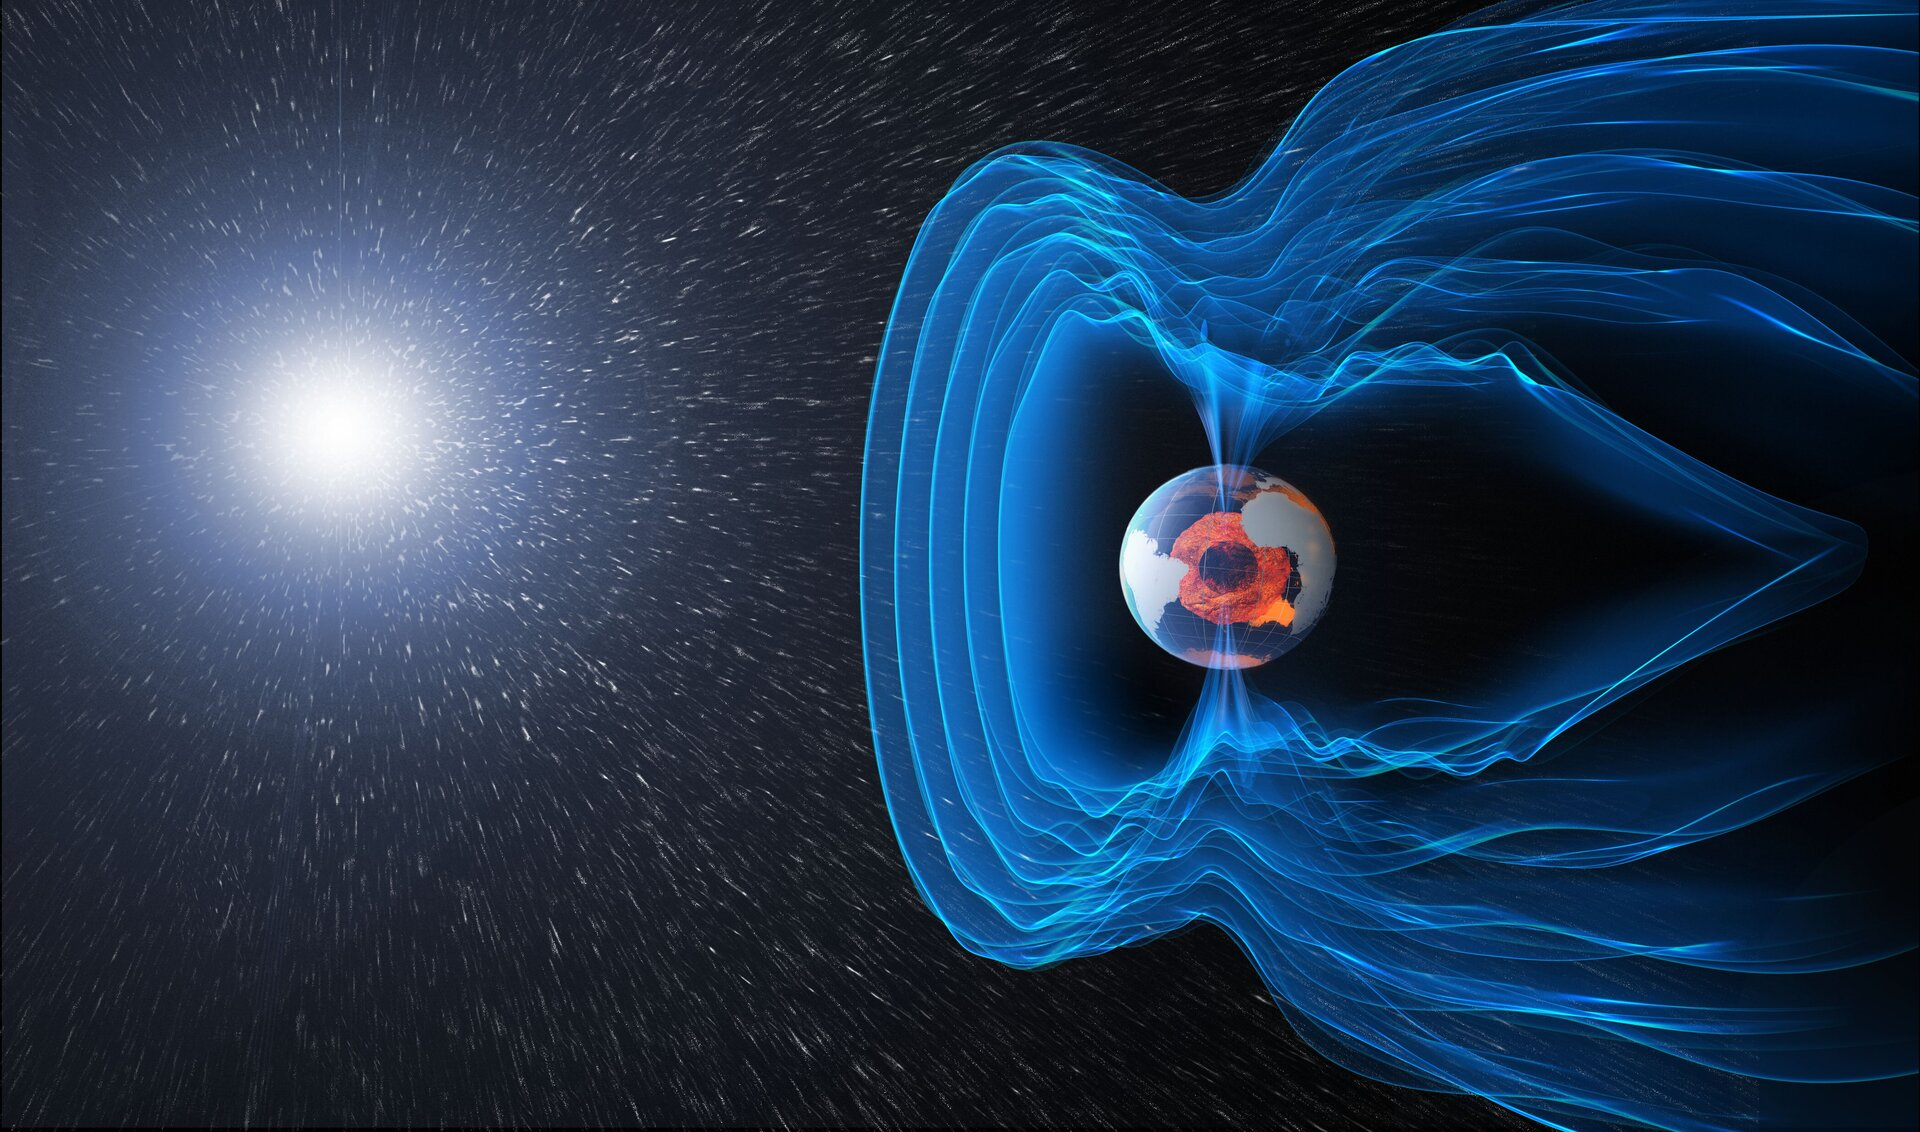
\includegraphics[width=1\textwidth]{images/cover1.jpg}
    \end{figure}

    % ---- Pousse le bloc suivant tout en bas de la page ----
    \vfill
    \noindent
    \begin{minipage}{0.48\textwidth}
        \raggedright
        Justine GARRAU \\         Pierre GUÉNO \\         Arthur LEBAS \\         Louann MONJARRET \\
        
    \end{minipage}
    \hfill
    \begin{minipage}{0.48\textwidth}
        \raggedleft
        Tuteurs : \\ Gautier NGUYEN \\ Antoine BRUNET \\ Guillerme BERNOUX
    \end{minipage}

\end{titlepage}

\setcounter{page}{2}
\section*{Remerciements}
\addcontentsline{toc}{chapter}{Remerciements}

merci tout le monde

\tableofcontents

\section*{Introduction}
\addcontentsline{toc}{chapter}{Introduction}


Nous allons parler de \acrlong{swx} et de \acrshort{ml}

\section*{Contexte Physique}
\addcontentsline{toc}{chapter}{1 - Contexte Physique}

\section*{État de l'Art}
\addcontentsline{toc}{chapter}{2 - État de l'Art}

\printbibliography %affichera la biblio quand on aura insérer notre .bib
\addcontentsline{toc}{chapter}{Bibliography}




Cover Photo: 












\addcontentsline{toc}{chapter}{Acronyms and abbreviations}
\begin{multicols}{2}
\printglossary[type=\acronymtype, nonumberlist]
\end{multicols}



\addcontentsline{toc}{chapter}{Glossary}
\label{sec:glossary}
\printglossary[nonumberlist]








\end{document}

